%!TEX root = ../../dissertation.tex
%%%%%%%%%%%%%%%%%%%%%%%%%%%%%%%%%%%%%%%%%%%%%%%%%%%%%%%%%%%%%%%%%%%%%%%%%%%%%%%%
%%%%%%%%%%%%%%%%%%%%%%%%%%%%%%%%%%%%%%%%%%%%%%%%%%%%%%%%%%%%%%%%%%%%%%%%%%%%%%%%
%%%%%%%%%%%%%%%%%%%%%%%%%%%%%%%%%%%%%%%%%%%%%%%%%%%%%%%%%%%%%%%%%%%%%%%%%%%%%%%%
\section{Streaming Modeling}
\label{c3:sec:modeling}

As stated, the goal of this chapter is to model the measuring process and reliable streaming. This section will introduce our reliable \gls{TCP}-based streaming model. It is intended for easily comparing different protocol variants against each other and measuring all variants in one testbed. 

But first, because any evaluation of a model requires metrics, we describe ones appropriate to the model and give a rationale.
 
%%%%%%%%%%%%%%%%%%%%%%%%%%%%%%%%%%%%%%%%%%%%%%%%%%%%%%%%%%%%%%%%%%%%%%%%%%%%%%%%
\subsection{Metrics for Reliable Transport Streaming}
\label{c3:metrics}

When measuring anything related to video or even just image quality, one has the choice between conducting a subjective or objective assessment. 

During a subjective test, human assessors evaluate and rate video quality in a controlled environment with the results usually being aggregated into an overall relative quality score \gls{MOS}. Through the human element, conducting a subjective assessment is very time and resource consuming but it also achieves the highest precision.

This is where, objective video quality assessments come into play. Modern objective models attempt to recreate the features of the humans' visual perception and psychophysics and are calibrated by subjective assessments. Most objective models operate on a full reference approach, they directly compare the original reference video to the resulting video after being encoding or transmitted.

Two of the simplest full reference image quality metrics, which can also be applied on video, are the \gls{MSE} and \gls{PSNR}, defined as:

\begin{equation}
    \begin{aligned}
    MSE = \frac{1}{N} \sum_{i=1}^{N}(x_i - y_i)^2\\
    \text{and } PSNR = 10 \log_{10} \frac{L^2}{MSE},
    \end{aligned}
\end{equation}

with $N$ as the number of pixels in a frame and individual pixels $x$ and $y$ from the reference and output frame respectively. $L$ denotes the maximum value of a pixel. For grayscale or when investigating each color channel separately, usually $L = \SI{8}{\bit} = 255$.  \cite{objective-vqa}

Image quality models can by nature only test for spatial distortions of a single image. This includes a general blockiness or blurriness, noise, or reduced resolution. Dedicated video quality assessments can additionally take temporal metrics into account, e.g. frame rate anomalies. Such models are being researched and standardized by the \gls{ITU} and \gls{VQEG} for example in \cite{ituJ144, ituJ246, ituJ247}.


When conducting dedicated streaming quality measurements, only this portion should be taken into account by a metric, and not the initial encoding process. During streaming only a specific subset of quality degradations can occur. Lost or late packets can cause missing blocks in a frame or frames to be skipped completely. Initial thoughts concerning \gls{IPTV} \gls{QoE} have been given in \cite{ituG1080} and the influence of packet delay variations on playout buffers is investigated in \cite{rfc3393}The \gls{MDI} \cite{rfc4445} is an attempt to capture this behavior and relate it to the network \gls{QoS}. Its metric relies on two properties, the \gls{DF}, as a measure of the network's latency and jitter, and the media loss rate. Of special interest to this investigation is the \gls{DF}, which is calculated based on a virtual buffer (VB) of received stream data as

\begin{equation}
    \begin{aligned}
        VB = r_{rcv} - r_{drain} \\
        DF_i = \frac{\max(VB) - \min(VB)}{r_{drain}}
    \end{aligned}
\end{equation}
 
Reliable streaming has even less possibilities to degrade a video stream. Packets can not be out of order and loss is concealed by \gls{TCP}, meaning that the transmitted and the played video are identical. The only thing that can still happen, is portions of the video arriving too late to be played out at their intended point in time.
A potential reliable streaming quality assessment metric needs to keep track of the following properties:

\begin{itemize}
    \item The initial delay, which is the time delta between the start of the transmission and the start of the video play.
    \item The number and lengths of interruptions or stalls during playback.
    \item For adaptive streaming, the characteristics of the quality levels the video was played in. This includes the number of switching events and the duration of each level.
\end{itemize}

A concise metric covering all properties has not been defined yet. The \gls{CI} was defined in \cite{1498486} and used to determine quality in \gls{P2P} live streaming. It is defined as \enquote{the number of segments that arrive before or on playback deadlines over the total number of segments} and with this partly captures the stalling property. In \cite{5634160} and \cite{DBLP:journals/corr/SeyedebrahimiBP13} a so-called \gls{PI} is defined and evaluated. The definition $I_p = uv$ is simply based on the number of stalls $u$ and the average stall duration $v$. 

Generally, most research operates just directly on these three properties, which allows for the most freedom in usage scenarios. The streaming measurement model presented in the following section also works with the assumption, that only the three properties are of importance. The model assumes no special metric, the individual properties can be directly attained from the model. Though any metric could still be applied on the results.


%%%%%%%%%%%%%%%%%%%%%%%%%%%%%%%%%%%%%%%%%%%%%%%%%%%%%%%%%%%%%%%%%%%%%%%%%%%%%%%%
\subsection{Measurement and Playback Model}
\label{c3:model}

Parts of the model presentation is based on the author's previous work published in \cite{cs3518}, \cite{metzger2011delivery}, and \cite{6229739}. It is based on the desire to compare all in-the-wild variants of reliable streaming protocols in a simple and concise way. This is achieved by basing the model on the component that is common to all of the approaches: the playback buffer.

To display a video stream, an application needs to maintain a playback buffer of sufficient size to at least gather enough data to reconstruct one single atomic unit of playback such as a video frame.
From the perspective of a player application , a video consists of a sequence of atomic units, video frames and audio samples.
The application progressively decodes the video from a source and stores the units temporarily in a memory buffer before playing them. In reliable streaming, the buffer is filled by the payload from received \gls{TCP} segments a subject to the network \gls{QoS}. The process can be subsumed as:

\begin{equation*}
\mathit{buffer}(t) = \sum_{0}^{t} \text{data}_\mathrm{received} - \sum_{0}^{t} \text{data}_\mathrm{played}
\end{equation*}

Both the incoming and outgoing data stream are variable over time. The fill level of the playback buffer is the critical component in the playback process and the central element of the model.If the buffer reaches a size of zero the playback process stops and stalling occurs.

\begin{figure}[htb]
    \centering
    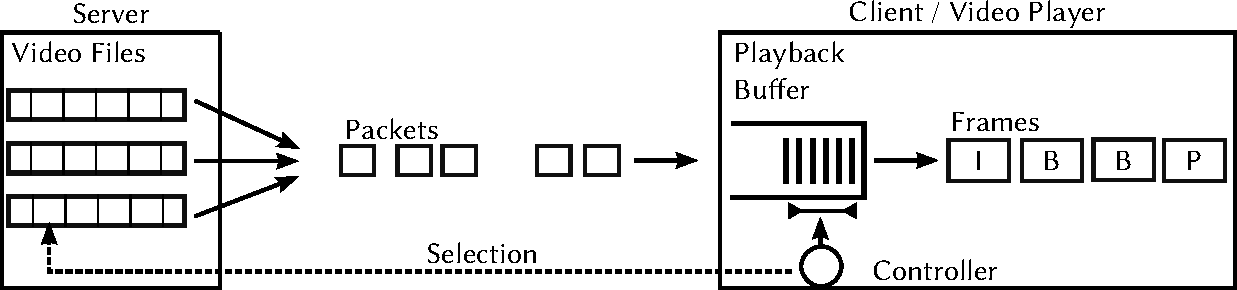
\includegraphics[width=0.9\textwidth]{images/playback-model.pdf}
    \caption{Reliable streaming playback model based on buffer control.}
    \label{c3:fig:playback-model}
\end{figure}

Figure~\ref{c3:fig:playback-model} overviews the reliable streaming model. The controller, part of the video player, selects a video from a remote location and the transmission is started, filling the playback buffer. The model has three degrees of freedom, which are all governed by the controller and together are coined playback strategies. These are:

\begin{itemize}
    \item The initial playback delay, which is the time between the initiation of the video stream transmission and the actual stream playback. The larger this is chosen, the bigger the safety margin on the buffer gets. If the video and transmission bitrate are known to be constant and and appropriately dimensioned, the initial delay can be chosen to be very small.
    \item Playback pause and resume decisions based on the current buffer fill level. This is a generalization of the initial playback delay, which is in fact only one, albeit always occurring stalling period.
    \item Selection of the video or video segment with a video bitrate chosen according to the current network throughput. This is only applicable for adaptive streaming.
\end{itemize}


These decisions yield a stalling period distribution for a streamed video. The frequency and the duration of stalls directly relate to the decision function of the playback model. The more frequent the stalls are, the shorter they will be; if the strategy produces longer stalls, they will be less frequent assuming the same network conditions. The time scale on which streaming applications buffer content usually lies in the range of seconds. This is a necessity in best-effort networks, as the available network bitrate might drop unexpectedly and cause stalling.


The the rest of this sections present fundamental playback strategies and strategy building blocks with features extracted from real world examples, which are given afterwards. 



%%
\subsubsection{Null Strategy}

The simplest strategy is having no strategy at all. Playback is started immediately when at least a single frame fully resides within the buffer and stops again at an empty buffer. The behavior can be summarized as ``Whenever anything can be played from the buffer, do so''.

This results in frequent stops and a large loss in playback continuity and will therefore not be used in practice. However, this strategy has some interesting theoretical properties, which is why it is mentioned here.
It minimizes total stalling time and the required buffer space. Moreover, it gives an upper limit for the number of stalls occurring\footnote{As a video frame is atomic, no other model could possibly stop the playback more often.}. Therefore, it can act as a baseline reference to assess the performance of other strategies.

\begin{figure}[htb]
    \centering
    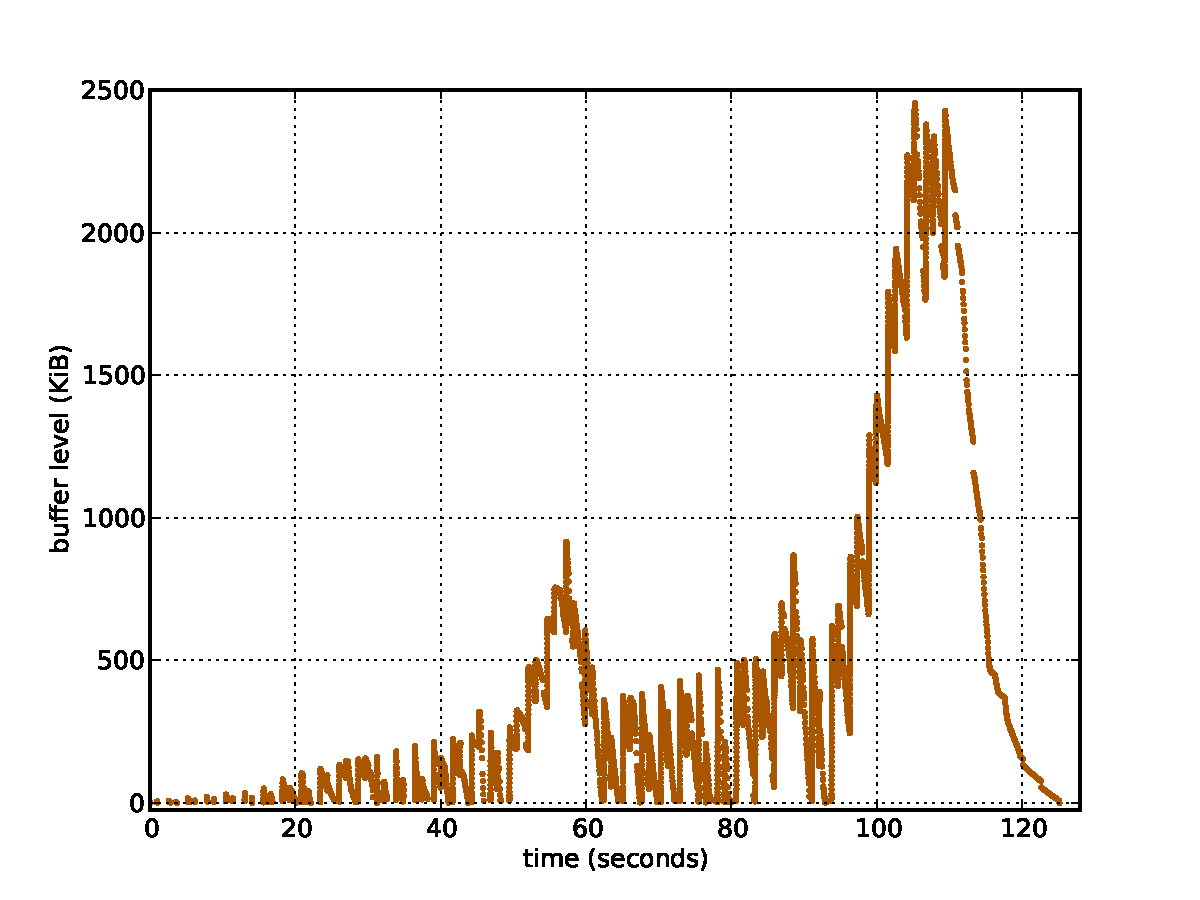
\includegraphics[width=0.9\textwidth]{images/bufferlevel-stall-new.pdf}
    \caption{Buffer fill level for the playback stalling model, \SI{33}{\second} total stalling.}
    \label{c3:fig:bufferlevel-stall}
\end{figure}

Figure~\ref{c3:fig:bufferlevel-stall} depicts an exemplary time series diagram of the contents of a video buffer using this strategy with a transmission rate only slightly above the video stream's rate. The buffer frequently drops down to zero forcing a short stall. According to the presented related work on the \gls{QoE} impact of stalling frequency in comparison to the length of stalls \cite{6123395}, this is the worst possible scenario for a person watching the stream.


%%
\subsubsection{Threshold Strategies}

Instead of instantly restarting playback, a lower threshold can be introduced. Only after a certain buffer fill level threshold has been surpassed, playback will be started. Thresholds can be set independently for the initial playback delay and stalls, with the initial playback delay generally set to be higher.

The threshold can be chosen in a number of ways. It can either be an absolute data volume, a buffered video duration. The latter is much more suited for variable bitrate videos as it automatically adapts itself to the current bitrate. A third option is to buffer for a certain amount of real time -- this can be seen as threshold -- and starting playback after that period regardless of the volume of the buffer. Additionally, the threshold could also either be set to a constant value or dynamically chosen according to the expected network \gls{QoS}.

Besides this single-threshold strategy, a two-threshold strategy might make more sense for segment-based streaming. In addition to the lower threshold, an upper threshold is introduced. When reached, no new segments will be requested until the buffer arrives at the lower threshold, or at an additional third threshold somewhere between the lower and upper bound, again. 

This model tries to resemble the playback mechanisms as implemented in YouTube's Flash video player.
It defers the start until at least two seconds of video data are buffered. When a stall occurs the player buffers at least five seconds of video before restarting. The model does not use any knowledge about the transmission (e.g. current bandwidth).
The result can be seen in Figure \ref{c3:fig:bufferlevel-flash}. Compared to the simple stalling model it increases the playback stability while only marginally affecting the total stalling time, resulting in 34 seconds of stalling.

\begin{figure}[htb]
    \centering
    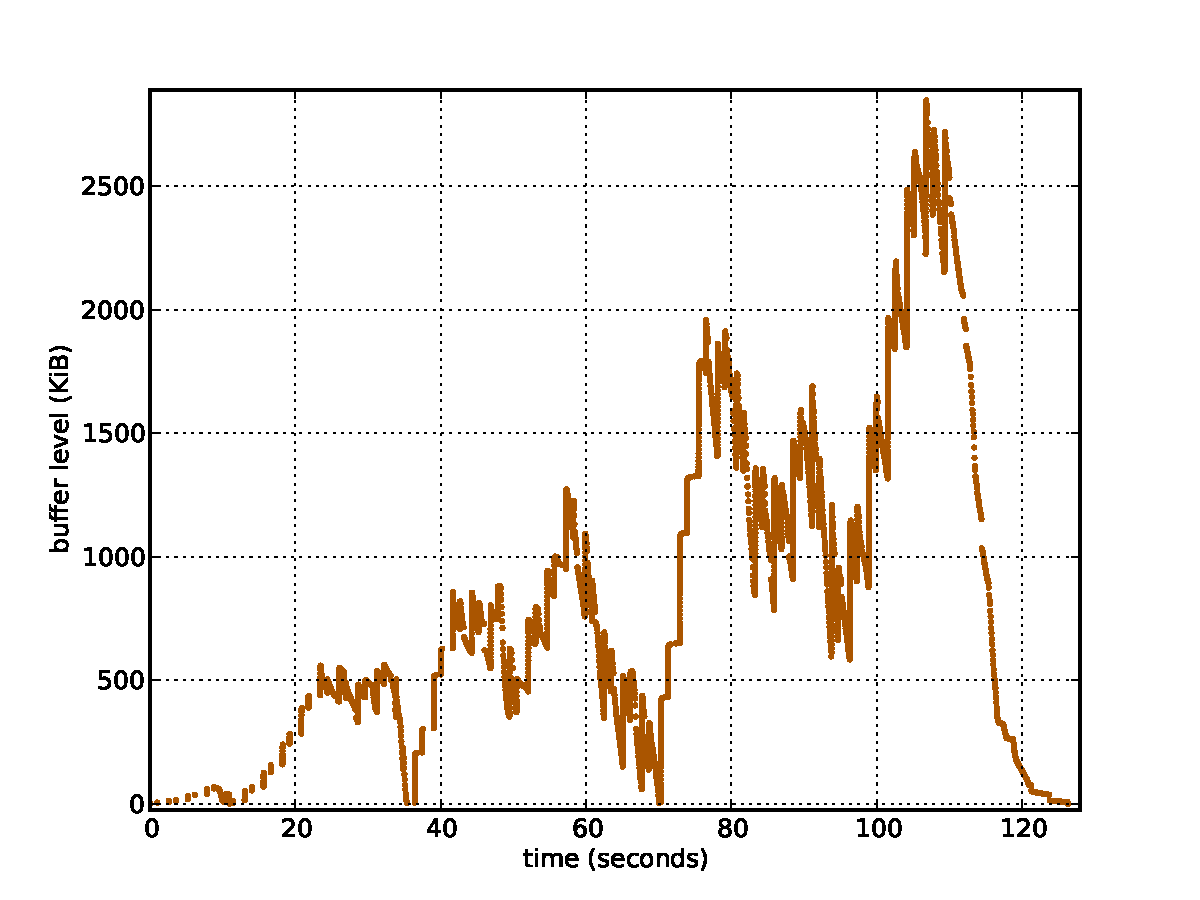
\includegraphics[width=0.9\textwidth]{images/bufferlevel-flash-new.pdf}
    \caption{Buffer fill level for the YouTube Flash Player model, \SI{34}{\second} total stalling.}
    \label{c3:fig:bufferlevel-flash}
\end{figure}


%%
\subsubsection{Predictive Strategies}



%%
\paragraph{Feedback Adaptive Model}

not only stalling characteristic but also a quality level distribution

Another user parameter is the quality level of the video for adaptive streaming. This trades off between maintaining a certain quality level and putting up with increased waiting times, and dropping the quality to a level sustainable at the current transmission rate.

adjustments to adaptive model: needs feedback loop to adjust quality
The model could also be extended to accommodate adaptive streaming mechanisms that feed back the buffer level to influence the download strategy of the player, e.g. send a receiver report to request a lower-bitrate stream in the case of RTP. % Consequently, the progress of data received would increase at a lower rate, and the playback rate would decrease as well once the residual stream data in the buffer were played out.



\subsubsection{Conditional and Combination Strategies}

    keep buffer between two thresholds // simpler version keep above one threshold
    measure


\subsubsection{Real World Implementation Examples}

The stalling and initial delay models define the maximum achievable upper and lower limits for the stalling parameter space for all possible real models.

The application behavior represents a trade-off between different types of perceivable artifacts -- initial startup delay, stalls, (partial) media skips (e.g. continuous audio, but skipping video), and quality adaption. The next Section will specifically look at these issues.

\subsubsection{Measuring the Model}

   Multiple incarnations of media streaming, but similar and (most of all!) comparable concepts and mechanisms => no need to assess single, specific protocols, networks, codecs, etc., but measure and describe generic, universal, common behavioral patterns => model, compare performance based on behavioral, structural commonalities. Choose for example a (range of) timescale(s) to find sets of mechanisms you need to look at. First use case to show how our system works: Progressive HTTP streaming. Will show adaptability to adaptive streaming and different protocols.

Directly measuring these two factors in a user-controlled browser does have drawbacks. The need for user interaction would hamper the effort of creating fully automated measurement series and getting reproducible results. Interfacing with the closed-source Flash software and getting meaningful results can also be a large hurdle.

To achieve increased flexibility we created several models that emulate the streaming process and its buffering and playback behavior. These are based on typical user playback solutions, e.g. a Web browser with a Flash plug-in. For this comparison we used a video of about 90 seconds length and network conditions that could not fulfill the video bitrate in time and hereby forced stalling to occur.


%% <-- WIP




%% <-- %% end WIP





%%
\subsubsection{Simple Predictive Model / Initial Playback Delay Model}

The second approach in Fig. \ref{c3:fig:bufferlevel-startdelay} defers the playback start as long as it is needed to play the video uninterrupted, meaning that the playback buffer will never run out of data. However, this approach is only viable with a complete knowledge over the downloading process, which can only be estimated in live scenarios. Because playback is done with global knowledge and at the earliest point possible the total stalling time is also 33 seconds, but only one long stalling phase occurs while the user initially waits for the playback to start.

The model is similar to progressively downloading the whole stream, as it will simply delay the initial start of the video until it can be played completely without any buffer underruns occurring. The only stall occurring is the initial waiting period until the video starts. The time spent waiting will also be minimal. The downside of this model is its use of perfect knowledge on the future network conditions at any point in time, making it purely theoretical. Actual streaming players need to accurately predict the transmission process, e.g. through moving averages.

\begin{figure}[htb]
    \centering
    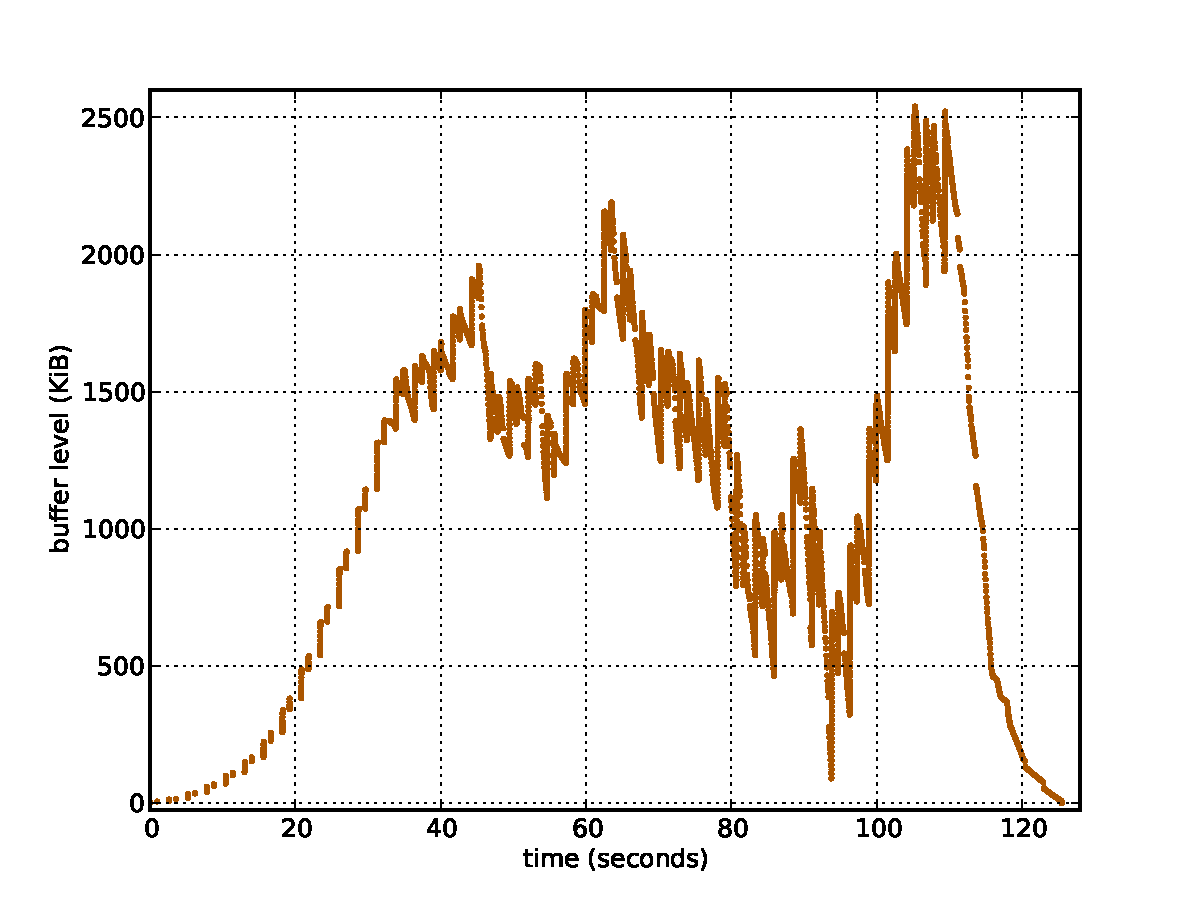
\includegraphics[width=0.9\textwidth]{images/bufferlevel-startdelay-new.pdf}
    \caption{Buffer fill level for the delayed playback model, \SI{33}{\second} total stalling.}
    \label{c3:fig:bufferlevel-startdelay}
\end{figure}


%%
\subsubsection{YouTube Flash Player Model}


This model is facilitated by the Flash Player used by the YouTube website. It will initially start the playback after it has buffered two seconds of video data. If a stall occurs it will restart playing after five seconds of video are in the buffer.
The Flash Model assumes sufficient network conditions in the beginning, requiring only a short initial playback delay to pre-fill the playback buffer. If, however, stalling occurs, then it will buffer longer to keep the stalling frequency down.




%%
\subsubsection{(Firefox) HTML5 Predictive Model}
The standard playback and buffering process of HTML5 is described in the HTML5 specification but adds up to:
\textit{``[...] the user agent [...] will automatically begin playback of the media resource as soon as it can do so without stopping.''} \cite{html5video}. The model presented here is based on the HTML5 implementation of the open source Firefox Browser in version 4 which differs slightly from the HTML standard. Because it is an online algorithm which does not have global knowledge of the video and transmission speeds of any point in the future it has to estimate these. It does so by calculating the moving averages of both. Playback is started when one of these conditions are met:

\begin{itemize}
\item The player has been buffering data for at least 30 seconds.
\item The player has already buffered an amount of data corresponding to 30 seconds of video.
\item The video download has been completed.
\item The moving average of the transmission rate is larger than the moving average of the video bitrate and the player has a safety buffer with 20 seconds of video data.
\end{itemize}

This approach is quite conservative and trades longer waiting times for fewer interruptions. The test case for our model is shown in Figure \ref{c3:fig:bufferlevel-firefox}. Initially, playback starts only after a long waiting period of about 25 seconds. Also, the only intermittent stall causes a long buffering period. Then again, the model keeps the total number of stalls down to this single stall. However, due to the longer overall stalling time of 44 seconds the player needs to buffer more data than the other model implementations. In our test case the maximum buffer size increased from about 2800 KiB to 5600 KiB. This may be a problem for devices with sparse amounts of memory, e.g. mobile telephones or small dedicated streaming boxes. However, a large buffer can also increase the chance of continuous playback in mobile scenarios with intermittent service interruption.

The algorithm used in the Firefox 4 browser is an approximate realization of the HTML5 video standard \cite{html5} which suggests starting the playback only when it can be ensured that the video can be played without interruption similar to the initial playback delay model.

The algorithm and its variables are shown in Algorithm \ref{c3:alg:firefox-PV} and Table \ref{c3:tbl:buffvars}, respectively. Firefox 4 uses moving averages to estimate the development of the transmission rate. It does not differentiate between intermittent and initial conditions. As the approach is similar in concept to the initial playback delay model, %it results in a very large required buffer space, but also %
it sports very few stalling events due to conservatively chosen (i.e., long) buffering times.



\begin{figure}[htb]
    \centering
    \begin{algorithmic}
        \IF {$s_{MA} > v_{MA}$} 
          \STATE $c \gets ( b_b=20s \lor b_T=20s )$
        \ELSE
          \STATE $c \gets ( b_b=30s \lor b_T=30s )$
        \ENDIF 
    \end{algorithmic}
    \caption{Firefox playback (re-)start decision algorithm.}
    \label{c3:alg:firefox-PV}
\end{figure}


\begin{table}[htb]
    \caption{Variables involved in buffering decisions.}
    \label{c3:tbl:buffvars}
    \centering
    \begin{tabu}{|l|X[p]|} 
    \hline
    Variable & Description \\ \hline
    $s_{MA}$ & Moving average of the transmission speed. \\
    $v_{MA}$ & Moving average of the video bitrate. \\ 
    $c$   & Condition upon which to start/resume playback. \\
    $b_b$    & Amount of video data the buffer contains. \\
    $b_T$    & Amount of time spent in non-playing buffering state. \\ \hline
    \end{tabu}
\end{table}
 
 \begin{figure}[htb]
    \centering
    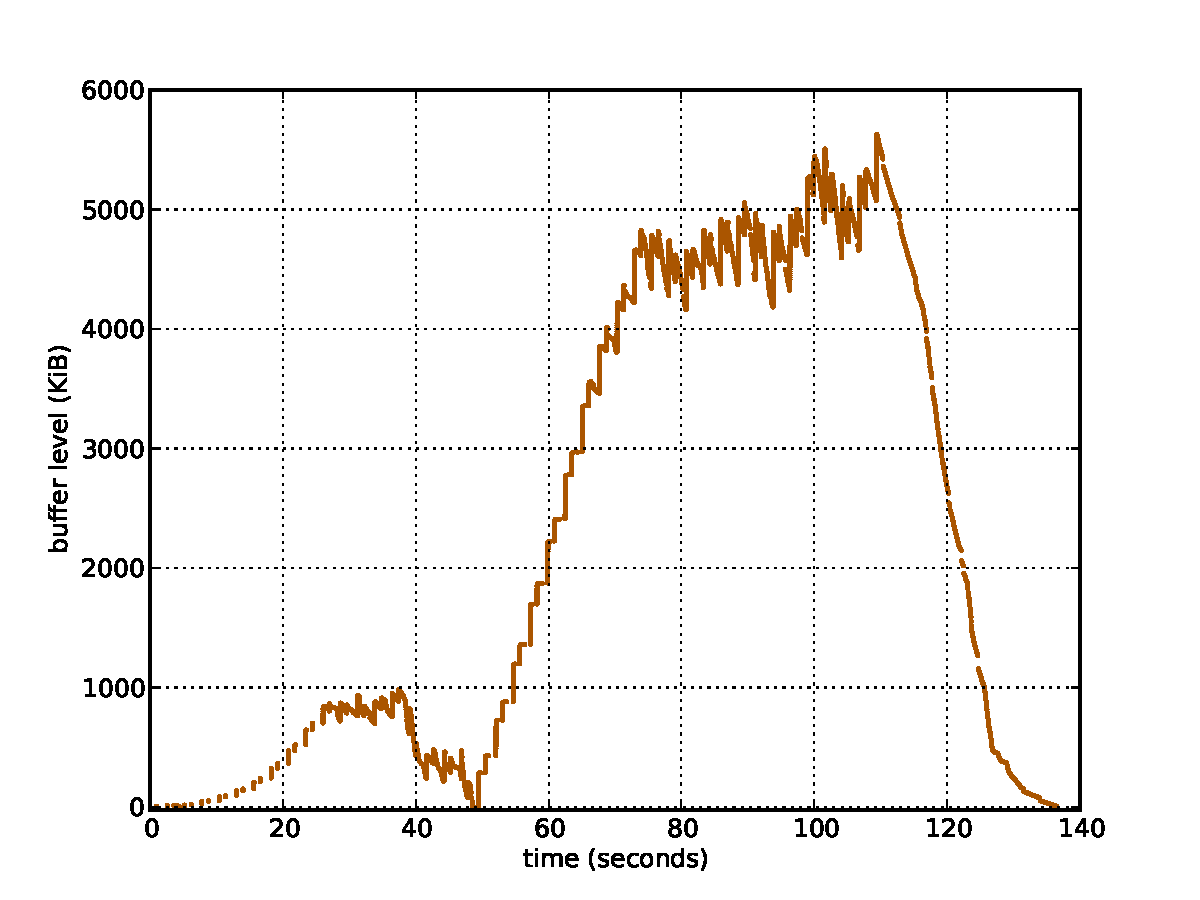
\includegraphics[width=0.9\textwidth]{images/bufferlevel-firefox-new.pdf}
    \caption{Buffer fill level for the Firefox 4 model, \SI{44}{\second} total stalling.}
    \label{c3:fig:bufferlevel-firefox}
\end{figure}




\subsubsection{Further Models and Variables}
In general, every streaming service practically implements its own playback model. Most of them will be very similar to the presented ones as the choices and parameters a streaming player has are rather limited.

For simple TCP streaming, the client can only influence the playback start and restart points after stalls. Adaptive streaming, i.e. streaming with the possibility of rate adaptation during playback, adds the choice of the quality and the number of segments to request in advance to control the fill level of the buffer.

Typical models for simple streaming will often try to set the current rates of the streaming transmission and the video in comparison to estimate if the buffer will continue to drain or fill. Depending on this variable an optimal buffering length can be calculated. The size should typically be larger if the transmission rate is not sufficient enough for the playback process to prevent frequent stalls.



% used yt-delay/hPUGNCIozp0_delay_2500 1, spyder, color #aa5500
% data
% start delay 33s 
% flash 33.82s
% stalling 32.68s
% html5 as implemented in firefox 44s


%Which offers better quality to users? Some approaches (TODO: refs and explain how)

% Longer waiting time but very few stops. Stalling model definitely the shortest waiting time but stops too frequent with insufficient network conditions, i.e. can not really be used. Delayed playback requires total knowledge not available beforehand. Can maybe used with reduced information, bandwidth estimation, but this is essentially HTML5/Firefox.




%``application comfort'' time to skip, ...
%\subsubsection{Unreliable Streaming Metrics}
%... and why they mostly do not work / are not applicable.